\section{Funções Polinomiais}
\begin{frame}
    \frametitle{Funções Polinomiais} 
    
    \begin{definicao}
    Diz-se que $p: \R \to \R$ é uma \sub{função polinomial} quando
    existem números reais $a_0, a_1, \dots , a_n$ tais que, para todo $x
    \in \R$, tem-se
    
    \begin{equation}\label{funcpol}
    p(x) = a_n x^n + a_{n-1} x^{n-1} + \dots + a_1 x + a_0.
    \end{equation}
    
    Os elementos de $\{x \in \R ; p(x) = 0\}$ são chamados de \sub{raízes de $p$}.
    \end{definicao}
    
    \end{frame}
    
    
    
    %------------------------------------------------------------------------------------------------------------
    
    \begin{frame}
    \frametitle{Funções Polinomiais} 
    
    \begin{exemplo}
    Além das funções lineares, afins e quadráticas, a soma e o produto
    de funções polinomiais são funções polinomiais. Considere a função
    polinomial $p$ tal que $$p(x) = \paren{x - \alpha} \paren{x^{n-1} +
    \alpha x^{n-2} + \dots + \alpha^{n-2}x+ \alpha^{n-1}}=x^n -
    \alpha^n.$$ Nesse caso, dizemos que $p(x)$ é \sub{divisível} por $x-
    \alpha$.
    \end{exemplo}
    
    \end{frame}
    
    
    
    %------------------------------------------------------------------------------------------------------------
    
    \begin{frame}
    \frametitle{Funções Polinomiais} 
    \begin{proposicao}
    Se $\alpha \in \R$ é raiz da função polinomial $p(x)$ de grau $n$,
    então existe uma função polinomial $q(x)$, de grau $n-1$, tal que
    $$p(x) = \paren{x- \alpha}q(x).$$
    Além disso, $p(x)$ não pode ter mais do que $n$ raízes.
    \end{proposicao}\pause
    
    Uma função polinomial $p$ chama-se \sub{identicamente nula} quando
    se tem $p(x) = 0$ para todo $x \in \R$. Nesse caso, $p$ tem uma
    infinidade de raízes, já que todo número real é raiz de $p$. Esse
    caso não contradiz a proposição anterior, já que o grau de uma
    função polinomial não está definido para a função identicamente
    nula.
    
    \end{frame}
    
    
    %------------------------------------------------------------------------------------------------------------
    
    \begin{frame}
    \frametitle{Funções Polinomiais} 
    \begin{teorema}
    Seja $p(x) = a_n x^n + a_{n-1} x^{n-1} + \dots + a_1 x + a_0$ uma função polinomial de grau $n$ e coeficientes inteiros. Se $\frac p q$ é uma fração irredutível e raiz de $p(x)$, então $p$ é divisor de $a_0$ e $q$ é divisor de $a_n$.
    \end{teorema}\pause
    
    Este Teorema nos permite encontrar facilmente as raízes racionais de um polinômio, caso exista alguma. Basta listar os divisores $p$ de $a_0$, os divisores $q$ de $a_n$ e testar se $p\paren {\frac p q }=0$ para todas as possíveis frações $\frac p q$. Caso haja alguma raiz racional de $p(x)$, ela estará entre as frações obtidas.
    
    \end{frame}
    
    %------------------------------------------------------------------------------------------------------------
    
    \begin{frame}
    \frametitle{Funções Polinomiais} 
    
    \begin{exemplo}
    Encontre todas as raízes do polinômio $p(x)=2x^4 +3x^3 +6x^2 +12x -8 = 0$.
    \end{exemplo}
    
    \end{frame}
    
    %------------------------------------------------------------------------------------------------------------
    
    \begin{frame}
    \frametitle{Funções Polinomiais} 
    \begin{proposicao}[Fórmula de Interpolação de Lagrange]
    Dados $n+1$ números reais distintos $x_0, x_1 , \dots , x_n$ e
    fixados arbitrariamente os valores $y_0, y_1, \dots, y_n$, existe
    um, e somente um, polinômio $p$ de grau menor ou igual a $n$ tal que
    $$p(x_0) = y_0, \ \ p(x_1) = y_1,  \dots , \ \ p(x_n) = y_n.$$
    
    $p(x)$ pode ser obtido pela fórmula:
    $$p(x) = \sum_{i=0}^{n} \colc{y_i \cdot \prod_{k \neq i} \paren{\frac {x-
    x_k}{x_i-x_k}}}.$$
    \end{proposicao}
    
    \end{frame}
    
    %------------------------------------------------------------------------------------------------------------
    
    \begin{frame}
    \frametitle{Gráficos de Funções Polinomiais} 
    Quando se deseja traçar o gráfico, ao menos um esboço, de uma função
    polinomial, certas informações são de grande utilidade. Listaremos
    algumas delas.
    
    Seja $p(x) = a_n x^n+ a_{n-1} x^{n-1} + \dots + a_1x + a_0$, com
    $a_n \neq 0$.
    \begin{itemize}
        \item Se $n$ é par, então para $\modu x $ suficientemente grande,
        $p(x)$ tem o mesmo sinal de $a_n$;
        \item Se $n$ é ímpar, então $p(x)$ tem o mesmo sinal de $a_n$ para
        valores positivos  muito grandes de $x$ e tem o sinal oposto de
        $a_n$ para valores negativos muito grandes, em módulo, de $x$.
    \end{itemize}
    
    \end{frame}
    
    %------------------------------------------------------------------------------------------------------------
    \begin{frame}
    \frametitle{Gráficos de Funções Polinomiais} 
    \begin{exemplo}
    Identifique se $n$ é par ou ímpar e qual o sinal de $a_n$ para cada
    um dos gráficos de funções polinomiais $p(x) = a_n x^n+ a_{n-1}
    x^{n-1} + \dots + a_1x + a_0$ abaixo:
    
    \begin{center}
    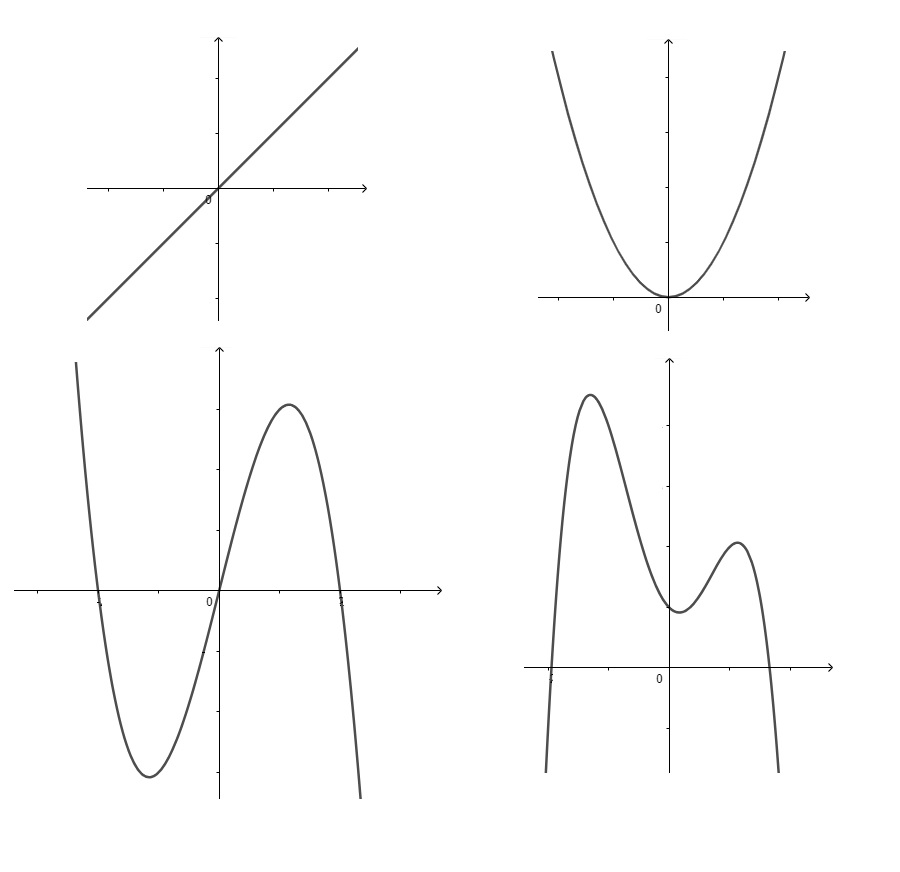
\includegraphics[width=5.8cm]{figures/4graf.jpg}
    \end{center}
    \end{exemplo}
    
    \end{frame}
    
    %------------------------------------------------------------------------------------------------------------
    \begin{frame}
    \frametitle{Gráficos de Funções Polinomiais} 
     Sejam $p$ e $q$ dois polinômios.
    
    \begin{itemize}
        \item Se o grau de $p$ é maior do
        que o grau de $q$, então para todo $x$ com valor absoluto
        suficientemente grande, tem-se $\modu {p(x)} > \modu{q(x)}$;
        \pause
        \item Sejam $x_1, x_2 \in \R$. Se $p(x_1) < 0$ e $p(x_2)>0$,
        então,
        $p$ deve possuir uma raiz entre $x_1$ e $x_2$.
    \end{itemize}
    
    \end{frame}
    
    %------------------------------------------------------------------------------------------------------------
    \begin{frame}
    \frametitle{Gráficos de Funções Polinomiais} 
    \begin{exemplo}\label{exemfig}
    Considere os polinômios $p(x) = x^7 $ e $q(x)=x^3$. Quando $0< \modu
    x < 1$, temos que $\modu {p(x)} < \modu{q(x)}$. Porém, quando $
    \modu x > 1$, temos que $\modu {p(x)} > \modu{q(x)}$. Além disso, em
    ambos os casos, $p(-1) = q(-1) = -1 <0$ e $p(1) = q(1) = 1 >0$.
    Assim, os polinômios possuem, cada um, ao menos uma raiz no
    intervalo $(-1, 1)$ -- a saber, $x=0$.
    
    \end{exemplo}
    
    \end{frame}
    
    %------------------------------------------------------------------------------------------------------------
    \begin{frame}
    \frametitle{Gráficos de Funções Polinomiais} 
    \begin{block}{Exemplo \ref{exemfig} (Continuação)}
    
    
    \begin{center}
    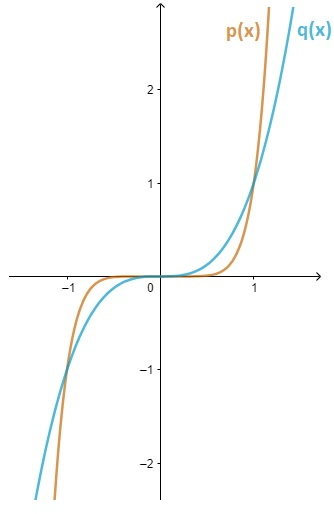
\includegraphics[width=4.3cm]{figures/2graf.jpg}
    \end{center}
    
    
    \end{block}
    
    \end{frame}
    
    %------------------------------------------------------------------------------------------------------------
